\documentclass[11pt, a4paper, german]{article}

\usepackage{booktabs}
\usepackage{algorithmic}
\usepackage[titlenotnumbered, vlined, ruled]{algorithm2e}
\usepackage{amsfonts}
\usepackage{amsmath}
\usepackage{amssymb}
\usepackage{amsthm}
\usepackage{mathtools}

\usepackage{array}
\usepackage[ngerman]{babel}
\usepackage[utf8]{inputenc}
\usepackage{color}
\usepackage{enumerate}
\usepackage{graphicx}
\usepackage{hyperref}
\usepackage{latexsym}
\usepackage{pdflscape}
\usepackage{makecell}
\usepackage{makeidx}
\usepackage{multirow}
\usepackage{pdfpages}
\usepackage{tikz}
\usepackage{tkz-fct}
\usepackage{tkz-graph}
\usetikzlibrary{patterns}
\usepackage{upgreek}
\usepackage{standalone}
\usepackage{slantsc}
\usepackage{lmodern}
\usepackage[labelformat=empty, font={scriptsize}]{subcaption}
\usepackage[labelformat=empty, font={scriptsize}]{caption}
\usepackage{pgfplots}
\usepackage{pgfplotstable}
\usepackage{circuitikz}
\usepackage{changepage}

\usetikzlibrary{shapes}
\usetikzlibrary{matrix, arrows,fit,shapes.gates.logic.US,shapes.gates.logic.IEC,calc,backgrounds,decorations.pathmorphing}




\DeclarePairedDelimiter\abs{\lvert}{\rvert}
\makeatletter
\let\oldabs\abs
\def\abs{\@ifstar{\oldabs}{\oldabs*}}
%
\let\oldnorm\norm
\def\norm{\@ifstar{\oldnorm}{\oldnorm*}}
\makeatother

\newcommand{\area}{\text{area}}
\newcommand{\uniquecone}{\text{unique\_cone}}
\newcommand{\uniquearea}{\text{unique\_area}}

\pgfplotsset{compat=1.8}

%
% Colors
%
\definecolor{darkblue}{RGB}{10, 0, 128}
\definecolor{grey}{RGB}{128, 128, 128}
\definecolor{darkred}{RGB}{180, 0, 0}
\definecolor{darkgreen}{RGB}{0, 100, 0}
\definecolor{lightgrey}{RGB}{210,210,210}
\newcommand{\RED}[1]{\textcolor{darkred}{#1}}
\newcommand{\BLUE}[1]{\textcolor{darkblue}{#1}}
\newcommand{\GREEN}[1]{\textcolor{darkgreen}{#1}}
\renewcommand{\emph}[1]{{\BLUE{#1}}}

\definecolor{darkRed}{rgb}{0.6,0,0}
\definecolor{lightRed}{rgb}{1,0.75,0.75}
\definecolor{darkGreen}{rgb}{0,0.5,0}
\definecolor{PineGreen}{rgb}{0.01,0.5,0.45}
\definecolor{darkBlue}{rgb}{0, 0, 0.75}
\definecolor{CornflowerBlue}{rgb}{0.15,0,0.7}
\definecolor{lightBlue}{rgb}{0.75,0.75,1}
\definecolor{grey}{rgb}{0.5,0.5,0.5}
\definecolor{black}{rgb}{0,0,0}
\definecolor{red}{rgb}{1,0,0}
\definecolor{green}{rgb}{0, 0.8, 0.3}
\definecolor{blue}{RGB}{10, 0, 128}
\definecolor{yellow}{rgb}{1,1,0}
\definecolor{orange}{rgb}{1,0.6,0}
\definecolor{cyan}{rgb}{0,0.7,1}
\definecolor{purple}{rgb}{0.5,0,0.8}

\newcommand\mycommfont[1]{\footnotesize\ttfamily\textcolor{darkGreen}{#1}}{}{}
\SetCommentSty{mycommfont}
\SetArgSty{textup}
\renewcommand\thempfootnote{\arabic{mpfootnote}}
\renewcommand{\thealgocf}{}

% \SetKwComment{Comment}{}{}

%
% Shorthands
%
\newcommand{\BL}{\textsc{BonnLogic}}
\newcommand{\Restr}{\textsc{And-Or}-Path Restructuring}
\newcommand{\AOP}{\textsc{And-Or}-Path}
\newcommand{\aop}{\textsc{And-Or}-path}

% \pgfpagesuselayout{resize to}[a4paper,landscape,border shrink=5mm]

% CONFIGURE PACKAGES

% NEW COMMANDS

\newcommand{\bl}[1]{\index{BonnLogic@\textsc{BonnLogic}!#1}}

\newcommand{\brent}[1]{\index{Brents adder@Brent's adder!#1}}

\newcommand{\ceil}[1]{\left\lceil #1 \right\rceil}

\newcommand{\delay}{\mathrm{delay}}

\newcommand{\depth}{\mathrm{depth}}

\newcommand{\floor}[1]{\left\lfloor #1 \right\rfloor}

\newcommand{\ld}{\log_{2}}

\newcommand{\loq}{\log_{\phi}}

\newcommand{\mini}[4]{\begin{minipage}{#1\linewidth}#3\end{minipage}\hfill\begin{minipage}{#2\linewidth}#4\end{minipage}}

\newcommand{\minialt}[4]{\centering{\begin{minipage}{#1\linewidth}#3\end{minipage}\begin{minipage}{#2\linewidth}#4\end{minipage}}}

\newcommand{\myindex}[1]{\emph{#1}\index{#1}}

\newcommand{\npfx}[1]{\index{non-prefix adders!#1}}

\newcommand{\OPT}{\mathrm{OPT}}

\newcommand{\pfx}[1]{\index{parallel prefix graph!#1}}

\newcommand{\size}{\mathrm{size}}

\newcommand{\sset}[1]{\left\{#1\right\}}

\newcommand{\todo}[1]{
  %\textcolor{red}{(TODO: \emph{#1})}
}

\newcommand{\vare}{\varepsilon}


% IMAGES

\newcommand{\tikzs}[2]{
  \centering
  \includegraphics[width=#1\linewidth]{images/#2.pdf} %fast
  %\ttikz{#2.tex}{#1} %slow
}
\newcommand{\tikzc}[3]{
  \centering{
    \includegraphics[width=#2\linewidth]{images/#3.pdf}
    \caption{#1}
    \label{fig:#3}%
  }
}
\newcommand{\tikzcc}[3]{
  \centering{
    \resizebox{#2\linewidth}{!}{
      \begin{tikzpicture}
        \input{images/#3}
      \end{tikzpicture}
    }
    \caption{#1}
    \label{fig:#3}%
  }
}
\newcommand{\ntikz}[1]{
  \begin{tikzpicture}
    \input{images/#1}
  \end{tikzpicture}
}
\newcommand{\ttikz}[2]{
  \centering{
    \resizebox{#2\linewidth}{!}{
      \begin{tikzpicture}
        \input{images/#1}
      \end{tikzpicture}
    }
  }
}
\newcommand{\ttikzfig}[3]{
  \begin{figure}[hbt]
    \centering{
      \resizebox{#2\linewidth}{!}{%
        \begin{tikzpicture}
          \input{images/#3}
        \end{tikzpicture}%
      }%
    }%
    \caption{#1}
  \end{figure}
}
\newcommand{\tikzfigs}[3]{
  \begin{figure}[hbt]%
    \centering{%
      \includegraphics[width=#2\linewidth]{images/#3.pdf}
      \caption{#1}%
      \label{fig:#3}%
    }%
  \end{figure}%
}
\newcommand{\tikzfigsc}[3]{
  \begin{figure}[hbt]%
    \centering{%
      \resizebox{#2\linewidth}{!}{%
        \begin{tikzpicture}
          \input{images/#3}
        \end{tikzpicture}%
      }%
      \caption{#1}%
      \label{fig:#3}%
    }%
  \end{figure}%
}
\newcommand{\tikzfig}[2]{
  \tikzfigs{#1}{1}{#2}
}


\usepackage{standalone}
\usepackage{slantsc}
\usepackage{lmodern}
%\newcounter{algorithm}
%\newtheorem{algorithm}[algorithm]{Algorithm}

\theoremstyle{plain}
\newtheorem{theorem}{Theorem}[section]
\newtheorem{cor}[theorem]{Corollary}
\newtheorem{lemma}[theorem]{Lemma}
\newtheorem{conj}[theorem]{Conjecture}
\theoremstyle{definition}
\newtheorem{definition}[theorem]{Definition}
\theoremstyle{remark}


\usepackage{caption}
\usepackage{subcaption}
\clubpenalty = 10000
\widowpenalty = 10000 
\displaywidowpenalty = 10000
\usepackage{Titelseite}
\usepackage{bbold}
\usepackage{graphicx}
\newcommand{\TM}{TechnologyMapping }

%Namen des Verfassers der Arbeit
\author{Alexander Zorn}
%Geburtsdatum des Verfassers
\geburtsdatum{26. Mai 1996}
%Gebortsort des Verfassers
\geburtsort{Bonn}
%Datum der Abgabe der Arbeit
\date{\today}

%Name des Betreuers
% z.B.: Prof. Dr. Peter Koepke
\betreuer{Betreuer: Prof. Dr. Stephan Held}
%Name des Instituts an dem der Betreuer der Arbeit tätig ist.
\zweitgutachter{Zweitgutachter: YYYY YYYY}
%z.B.: Mathematisches Institut
\institut{Forschungsinstitut f\"ur Diskrete Mathematik}
%Titel der Bachelorarbeit
\title{Heuristiken f\"ur das TechnologyMapping}
%Do not change!
\ausarbeitungstyp{Bachelorarbeit Mathematik}



\begin{document}

\maketitle

\tableofcontents
\newpage 
\section{Einleitung}

Der zunehmende Gebrauch elektronischer Geräte verlangt nach immer leistungsfähigeren Computerchips. Ein solcher wenige Quadratzentimeter große Chip beherbergt bis zu mehreren Milliarden Transistoren, welche, durch Drähte verbunden, gemeinsam eine Logische Funktion errechnen. Das Chipdesign beschreibt die Aufgabe aus einer gegeben Logischen Funktion einen herstellbaren Chip zu entwerfen, welcher diese Funktion realisiert. \\ 
\begin{wrapfigure}{r}{6cm}
	\scalebox{1}[-1]{
		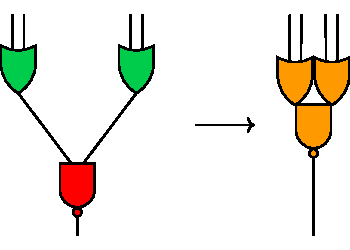
\includegraphics[]{pictures/compiled/einfBsp}
	}
		\caption{Zwei Realisierungen der Logischen Funktion $\neg((w\lor x) \land (y \lor z))$}
\end{wrapfigure}
Mithilfe von, aus wenigen Transistoren konstruierten, Bauteilen (genannt Gates, z.B.: AND, OR, INV, OAI) lässt sich eine Logische Funktion nachbilden. Abbildung 1 (links) zeigt dies an einem kleinen Beispiel.  Die Realisierung einer solchen Funktion ist jedoch nicht eindeutig, wie die in Abbildung 1 (links und rechts) gezeigte Nachbildung, beweist. \\
Die Größe der Menge aller möglicher Baupläne (später Circuit) für eine Logische Funktion hängt maßgeblich von der Anzahl der zur Verfügung stehenden Bauteile, sowie von dem Aufbau der Funktion, ab.
Es stellt sich heraus, dass im Allgemeinen eine Vielzahl möglicher Realisierungen einer Logischen Funktion existieren. Jedes Bauteil besitzt physikalische Eigenschaften an Größe, Geschwindigkeit (Delay) etc.. Somit besitzt auch jede Realisation solche Eigenschaften. \\
Ziel des \TM ist es für eine Logische Funktion eine Realisierung zu finden, welche eine Kostenfunktion (bestehend aus den physikalischen Eigenschaften) optimiert. Die Wahl der Implementierung hat direkte Auswirkungen auf die  Schnelligkeit, Größe und den Stromverbrauch des fertigen Chips. Hierbei geht das \TM von einer bereits realisierten Logischen Funktion aus und baut diese um zu einer möglichst kostengünstigen Alternative um. \\
Der optimale mögliche Umbau lässt sich bei kleinen oder eingeschränkten gegebenen Bauplänen noch in akzeptabler Zeit finden. Die Lösung dieses Problem für allgemeine Baupläne und Kostenfunktionen ist jedoch ein NP vollständiges Problem. Aus diesem Grund entwickelt die folgende Arbeit eine Heuristik, welche für sehr (mehrere 10.000 Bauteile) große Baupläne in akzeptabler Zeit einen möglichst kostengünstigen Umbau ermöglicht.\\
\textcolor{red}{am ende hier noch eine kurze Quellenübersicht geben an lukas orientiert}

\newpage

\section{Terminologie \& grundlegender Algorithmus}
\subsection{grundlegende Definitionen}
Es folgen ein paar grundlegende Definitionen zur Beschreibung des Problems.

\begin{definition}{Boolesche Variable und Funktion: } \\
Eine boolesche Variable ist eine Variable mit Werten in $ \{ 0 , 1 \} $.
Sei $ n, m \in \mathbb{N}$. Eine boolesche Funktion ist eine Funktion $ f : \{ 0 , 1 \}^n \rightarrow \{ 0 , 1 \}^m $ mit n inputs und m outputs. 
\end{definition}

\begin{definition}{Gate und Library:}\\
Ein Gate $g$ mit Eingangsgrad $ n \in \mathbb{N}$ ist ein Tripel $(f_g, d_g, area_g)$. Hierbei sind $d_g, area_g \in \mathbb{R}_{\geq 0}$. Des Weiteren gilt $f_g$ ist eine boolesche Funktion mit $ f_g : \{0,1\}^n \rightarrow \{0, 1\} $. \\
Eine Library L ist eine Menge von Gates und sei \\ 
$fanin_{max} := max\{ arity(g) | g \in L \}$.
\end{definition}
\begin{figure}[h]
\begin{center}
 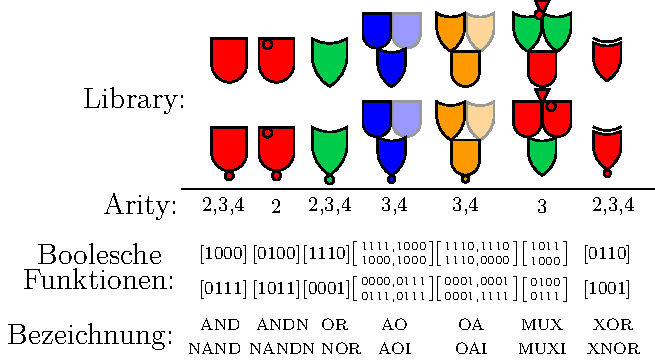
\includegraphics[height = 80pt]{./pictures/compiled/new_library.pdf}
 \caption{Beispiel einer Library}
 \label{fig:bsplib}
\end{center}
\end{figure}
$area_g$ gibt die Größe des physikalischen Bauteils an und $d_g$ beschreibt die Zeit die ein Signal braucht um von den inputs des Gates zu seinem Output zu gelangen. Dieser Wert lässt sich noch weiter differenzieren indem man $d_g \in \mathbb{R}^n$ wählt und somit Zeiten für jeden der Inputs angeben werden kann.\\

\begin{definition}{Circuit:}\\
Ein Circuit ist ein gerichteter kreisfeier Graph (directed acyclic graph DAG) mit folgenden Eigenschaften. Jeder Knoten gehört zu einer der aufgelisteten Kategorien: 
\begin{itemize}
\item{\bf Input} Knoten mit Eingangsgrad Null.
\item{\bf Gates} mit mindestens einer eingehenden Kante und ausgehenden Kante. Diese korrespondieren zu der Definition oben mit dem Zusatz dass an jedem der Inputs optional ein Inverter liegen kann.
\item{\bf Outputs} mit genau einer eingehenden Kante und keiner ausgehenden.
\end{itemize}
Ein Gate mit mehr als einer ausgehenden Kante wird auch Highfanoutgate genannt.\\
Ein Circuit realisiert durch Verschachtelung der booleschen Funktionen seiner Gates ebenfalls eine boolesche Funktion. \\
Zwei Circuits heißen äquivalent, wenn sie die gleiche boolesche Funktion realisieren.
\end{definition}

In einem Circuit lassen sich Teilgraphen durch ein Gate der Library austauschen. Voraussetzung für einen solchen Tausch ist, dass der veränderte Circuit äquivalent zu dem originalen ist. Dies sicher die folgenden Definitionen. 

\begin{definition}{Match und Kandidat:}\\
Sei g ein Gate in einem Circuit $C$. Ein (invertiertes) Match m ist ein Tupel $(p_m, I_m, f_m, inv_m)$ welches folgendes enthält:
\begin{itemize}
\item Ein Gate p der Library
\item Eine Menge X von Knoten aus der Circuit und eine Bijektion $ f: X \rightarrow inputs(p)$
\item Ein Funktion $ inv : inputs(p) \rightarrow \{not\_inv , inv \}$
\end{itemize}
So dass der Circuit $C'$, welcher durch den Austausch des Sub-Circuits von X bis g durch das Match (mit den durch inv definierten Invertern an den Inputs) entsteht, äquivalent zu C ist.
Ein invertiertes Match auf g ist ein Match auf g mit einem Inverter an jedem seiner Outputs.\\
Ein (invertierter) Kandidat auf g besteht aus einem (invertierten) Match auf g und einem Kandidaten für jeden Input Knoten von g (welcher kein Input von C ist).
\end{definition}

\begin{definition}{Circuit-Kandidat:}\\
Sei C ein Circuit mit Outputknoten Menge O. Eine Circuit-Kandidat K von C ist eine Menge von Kandidaten, sodass $\forall o \in O \, \exists!  h  \in K : h$ ist Kandidat von $ o$ und an jedem Knoten von C an dem sich mehrere Kandidaten überschneiden ist dasselbe Match gewählt.
\end{definition}
Folgendes Beispiel visualisiert die vorherigen Definitionen.\\
\textcolor{red}{BILD EINSETZEN}

Ein Circuit-Kandidat C ist eine Möglichkeit den Circuit physikalisch zu realisieren. Wie bereits in der Einleitung bemerkt gilt es nun den besten Kandidaten auf C auszuwählen. Dafür ist ein Maß für Implementierungen von Circuits notwendig. Es folgen zwei geläufige Beispiele. In der Praxis (und im späteren Verlauf dieser Arbeit) wird in der Regel eine convex-Kombination aus beiden verwendet.

\begin{definition}{Area und Delay eines Kandidaten:}\\
Sei C ein Circuit und K ein Circuit-Kandidat auf C. Dann gilt: \\
\begin{itemize}
\item $area(K) = \sum_{g \in gates(C)} (a_g + \sum_{i \in inputs(g)} \mathbb{1}_{\{inv_g(i)==inv\}} area_{inv})$ \\
wobei $area_{inv}$ die Größe eines Inverters ist.
\item $AT(K) = $\\$  \max\limits_{k \in can(K)} \{\max\limits_{i \in inputs(k)} \{   d_{gate(k)} + \mathbb{1}_{\{inv_g(i) \}} d_{i} + AT(inp\_can(k,i)) + d_{w(k,i)} \} \}$ 
\end{itemize}
Wobei $can(K)$ die Menge der Kandidaten von $K$ sind und $inputs(k)$ sind die Inputknoten des Outputknoten des Kandidaten k. Des Weiteren ist $d_i$ das Delay eines Inverters und $d_{w(k,i)} $ das Delay der Kante zwischen den Knoten $k$ und $i$. $inp\_can(k,i)$ gibt den Kandidaten des $i$'ten Inputs von k zurück. 

\end{definition}

Das Delay (AT) gibt an, wann das letzte Signal aus einem der Outputs des Circuit kommt.

\subsection{Kern Algorithmus}

Es folgt ein grundlegender Algorithmus, welcher auf eingeschränkten Circuits arbeitet, jedoch im weiteren Verlauf dieser Arbeit zu einer Heuristik für allgemeine sehr große Circuits erweitert wird.

\begin{problem}[framed]{(einfaches) Technology Mapping}
  Instanz:  & Circuit $C$ ohne Highfanoutknoten (Knoten mit nur einer ausgehenden Kante), mit eindeutigem Output $o$, Library $L$ mit beschr\"anktem $fanin_{max}$\\
  Aufgabe: &  Finde einen Kandidaten $K$ auf $o$, welcher die Arrivaltime/Area minimiert.
\end{problem}

\begin{algorithm}[H]
 \LinesNumbered
 \DontPrintSemicolon
 \caption{(einfaches) Technology Mapping}
 \SetKwInOut{Task}{Task}
 \KwIn{Circuit $C$ kreisfrei mit finalem Output $o$, Library $L$}

 bester\_kandidat[] $\gets \emptyset$\;
 bester\_inv\_kandidat[]$ \gets \emptyset$\;
 \ForEach{Knoten $v \in V(G)$ in topologischer Reihenfolge}
 {
   berechne alle (invertierten) Matches auf $v$\;
   \ForEach{ Match $m$ auf $v$ }
   {
      Berechne besten Kandidaten mit $m$ auf $v$\;
      Update best\_(inv)\_kandidaten\;
   }
 }
 Implementiere $C$ entsprechend bester\_kandidat[$o$]\;
\end{algorithm}\ \\

\begin{definition}{optimaler \TM Algorithmus:}\\
	Ein Algorithmus für das \TM auf einem Circuit $C$ heißt optimal, wenn er den (bzgl. der Kostenfunktion) besten äquvalenten Circuit $C'$ liefert, welcher durch das Anwenden der erlaubten Operationen auf $C$ konstruiert werden kann. 
\end{definition}
Daraus folgt, dass der Zusatz optimal abhängig davon ist, was die erlaubten Operationen sind.
Im Weiteren Verlauf der Arbeit werden weitere Operationen hinzugefügt und der Circuit verallgemeinert. Das Attribut optimal bezieht dann, wenn dies nicht dabei steht,  auf alle bisher vorgestellten Operationen. Zu diesem Punkt umfasst die Menge der erlaubte Operationen das logische äquvalente matchen von Subcircuits mit Elementen der Library.\\

Ein optimaler \TM Algorithmus liefert in der Regel nicht die bestmögliche Implementierung der $C$ zugrunde liegenden logischen Funktion.\textcolor{red}{dies lässt sich super anhand der redundant matche zeigen -> Bild!!} \\

\begin{cor}
	Das einfache \TM ist optimal. 
\end{cor}
\begin{proof}
	Der Algorithmus geht in topologischer Reihenfolge durch die Knoten $v$ des Graphen und berechnet alle Matche auf $v$. Diese werden dann zu einem Kandidaten ergänzt. 
 Ohne Highfanout-Knoten überschneiden sich diese nicht. Für jeden Knoten und jedes Match gibt es nur einen Kandidaten zur Auswahl, da für die Inputs des Matche jeweils nur ein Kandidat gespeichert wurde. An jedem Knoten wird nur das Match (mit dem dazugehörigen Kandidaten) gespeichert, welches die Kosten optimiert. \\
 Es bleibt zu zeigen, dass angenommen für alle Knoten mit kleinerem topologischen Rang als $rand(v)$ ist der bestmögliche Kandidat gespeichert, so wird, nach gerade beschriebenem Vorgehen, auch für $v$ der schnellste (bzw. kleinste) Kandidat $k$ gespeichert. \\
 Angenommen es gibt einen besseren Kandidaten $k'$, als $k$, welcher von dem Algorithmus gespeichert wurde. Sei $k''$ der Kandidate, welcher dasselbe Match wie $k'$ benutzt und die besten Input Kandidaten. Da $k''$ die besten Input Kandidaten benutzt ist er mindestens so schnell (bzw. klein) wie $k'$. $k$ ist jedoch ebenfalls mindestens so kostengünstig wie $k''$ (andernfalls hätte der Algorithmus $k''$, $k$ vorgezogen). Dies ist ein Widerspruch zur Annahme. 
\end{proof}
 
\begin{cor}{Der Algorithmus für das (einfache) \TM  \\ besitzt $\mathcal{O}(  |V(C)||L| fanin_{max})$-Laufzeit}
\end{cor}
\begin{proof}
Schritt 1 und 2 besitzen Laufzeit $\mathcal{O}(1)$. Schritt 4 lässt sich in \textcolor{red}{ wielange braucht es ein zu checken ob ein gate der Library ein Match eines Knoten sein kann ? ? plus Begründung! Laufzeit anpassen}. Schritt 6 ist wie bereits erwähnt schnell implementierbar, da für jeden der max $fanin_{max}$ Inputs der beste Kandidat verlinkt werden muss. Die Invertierten Matche werden nur gebarucht wenn der Input invertiert war. Somit braucht $\mathcal{O}(fanin_{max})$. Schritt 3 und 5 sind zwei verschachtelten Schleifen mit  $|V(C)|$ und max $|L|$ Durchläufen. \\
Daraus folgt eine Laufzeit von $\mathcal{O}(  |V(C)||L| fanin_{max})$.
\end{proof}



\newpage
\section{Allgemeiner Algorithmus und Heuristik}
\subsection{Tradeoffprobleme}
Der oben vorgestellte Algorithmus ist in der Lage den bestmöglichen Umbau eines eingeschränkten Circuits zu bezüglich Area oder Delay zu errechnen. \\
Es existiert  ein Tradeoff zwischen Area und Delay. Dies hat zur Folge, dass ein möglichst kleiner Circuit im Allgemeinen sehr langsam ist und man bei einer sehr schnellen Lösung mit einem großen Platzverbrauch rechnen muss. In der Anwendung des \TM ist jedoch weder ein sehr langsamer noch ein besonders grosser Circuit akzeptabel.\\
Daraus folgt die Nachfrage nach einem Algorithmus, welcher in der Lage ist bezüglich einer Konvexkombination oder einer Schranke zu optimieren. Daraus ergeben sich die beiden folgenden Optimierungs-Probleme: \\

 \begin{problem}[framed]{\TM mit Konvexkombination}
  Instanz:  & Circuit $C$,mit einem Output, Library $L$ mit beschr\"anktem $fanin_{max}$,
  $|L|$ beschränkt und  Tradeoff-Parameter $\lambda \in [0,1]$ \\
  Aufgabe: &  Finde einen Circuit-Kandidaten $K$ auf $C$, welcher $\lambda AT(K) +(1-\lambda )area(K) $ minimiert.
\end{problem}
 \begin{problem}[framed]{\TM mit Arrivaltimeschranke}
  Instanz:  &  Circuit $C$,mit einem Output, Library $L$ mit beschr\"anktem $fanin_{max}$,
  $|L|$ beschränkt und Arrivaltimeschranke $A_{max}$ \\
  Aufgabe: &  Finde den kleinsten Circuit-Kandidaten $K$ auf $C$, für den $AT(K) \leq A_{max}$ gilt, oder entscheide, dass für jeden Circuit-Kandidaten $K$ bereits $AT(K) > A_{max}$ gilt.
\end{problem}
Im weiteren Verlauf dieses Kapitels, werden diese Problemstellungen auf Circuits mit mehreren Outputs erweitert. \\

Diese \textcolor{red}{diese Probleme sind äquvalent Beweis? oder verweis aus quelle}
\textcolor{red}{erwähnen dass da die äquivalent sind von nun an nur noch die Konvexkombination verwendet wird}

Dadurch ergibt sich folgende Problemstellung für den Algorithmus: \\
Angenommen an jedem Knoten $v$ würde, wie im Kern-Algorithmus, nur derjenige Kandidat gespeichert werden, welcher die Kostenfunktion an $v$ optimiert. Dadurch kann nicht mehr garantiert werden, dass beim errechnen der Kandidaten für den Output, der für ihn optimale Kandidat noch vorhanden ist. Dies beweist das Beispiel in Abbildung \textcolor{red}{hier abb einfügen}. Beide Inputs getrennt nach der Kostenfunktion zu optimieren, garantiert offenbar nicht das optimale Ergebnis.\\

Die Kosten eines Kandidaten k sind somit nicht $\lambda AT(k) +(1-\lambda )area(k)$,  sondern das Tupel $(AT(k), area(k))$.
Es gibt jedoch eine Klasse von Kandidaten, welche nicht gespeichert muss. Dazu folgende Definition\\

\begin{definition}{(dominierte Kandidaten)}\\
	Seien $k_1, k_2$ Kandidaten desselben Knotens. Dann wird $k_1$ von $k_2$ dominiert, wenn gilt:\\
	$AT(k_1) < AT(k_2) und area(k_1) \leq area(k_2)$\\
	$	AT(k_1) \leq AT(k_2) und area(k_1) < area(k_2)$\\	
\end{definition}

Eine optimale Lösung des \TM verwendet offenbar (\textcolor{red}{in einem Korollar beweisen ?}) nur nicht-dominierte Kandidaten, woraus folgt, dass nur diese während der Ausführung des Algorithmus gespeichert werden müssen.\\
Die Menge der noch bleibenden Kandidaten lassen sich in sogenannten Tradeoff-Kurven speichern (siehe Abbildung ?? \textcolor{red}{Abbildung hinzufügen.. kann ich Lucas verwenden ?}). Welche jeden Kandidaten zweidimensional anhand seiner Kosten erfasst.\\

Die beiden vorgestellten Probleme sind NP-vollständig. Daraus folgt, dass sich ab diesem Punkt wahrscheinlich  kein polynomieller optimaler Algorithmus für das \TM finden lässt. Dadurch dass sich zwei Kandidaten in den meisten Fällen nicht mehr vergleichen lassen, wird eine Vielzahl von Kandidaten an jedem Knoten gespeichert. Dies zeigt sich in einem exponentiell großen Speicheraufwand.  \textcolor{red}{hier könnte lukas FPTAS auch hin}\\
Einen Beweis der NP-vollständigkeit findet sich in \textcolor{red}{hier den verweis zu einem Beweis einfügen}.

\subsection{Highfanoutknoten}
Der oben beschriebene Kern Algorithmus arbeitet nur auf Circuits, in denen keine Highfanoutknoten existieren. Diese Eigenschaft kommt auf einem realen Chip jedoch sehr häufig vor(ca. 25\% der gesamten Knoten sind Highfanoutknoten für einen genaueren Zusammenhang von der Anzahl der Highfanoutknoten und der Laufzeit siehe das Kapitel 8).\\
 Es ist möglich einen Circuit, in kleinere Subcircuits zu unterteilen, welche solche Highfanoutknoten nicht besitzen. Die Subcircuits werden daraufhin einzeln mit dem Algorithmus (sehr schnell) optimiert und daraufhin zu einem C äquvalenten Circuit C' zusammengesetzt. Diese Vorgehensweise findet sich ausführlich in \textcolor{red}{Hier das eine Paper suchen plus einfügen} wieder. Die folgende Abbildung verbildlicht diesen Ansatz einer Heuristik. \textcolor{red}{Bild erstellen, welches sich an dem des Papers orientiert}.\\
  Der Anteil an Highfanoutknoten ist auf den mir vorliegenden Chips so groß, dass eine vielzahl sehr kleiner Subcircuits mit einer somit kleinen Anzahl an Kandidaten entstehen, woraus folgt, dass die Möglichkeiten des \TM sehr eingeschränkt werden. Aus diesem Grund werde ich auf diese Art der   Heuristik nicht mehr eingehen.\textcolor{red}{zu anna gibt es sonst noch einen grund dies nicht doch einmal auszuprobieren?}\\

\textcolor{red}{Klonen erwähnen? (aktuell wird sie nicht erwähnt (mit beispiel bild ? machen! in der definition des Circuit Kandidaten wurde das extra weggelassen}\\

Das Kern-Problem der Highfanoutknoten ist, dass bei der Konstruktion des äquivalenten Circuits die eingebauten Kandidaten aller Nachfolger eines Highfanoutknoten $v$ an $v$ übereinstimmen müssen. Daraus folgt, das bei der Wahl eines Kandidaten für einen Knoten w die Wahl der Kandidaten der Input-Kandidaten von w nicht unabhängig von einander sein muss. \\
Zur Lösung des Problems helfen die folgenden Definitionen:\\

\begin{definition}{Cone eines Knoten:}\\
	Sei C ein Circuit und v ein Knoten von C. Dann sei die Cone von v: 
	\[ cone(v) := C[V \cup \{ v \}], V = \{ w \in V(C) : \exists \text{ w-v-Weg in }  C \} \] 
\end{definition}
\textcolor{red}{Bild ? }

\begin{definition}\  \\
	Sei C ein Circuit und  $v \in V(C)$. Dann wird die durch $cone(v)$ berechnete Funktion. Die 			{\bf bis v berechnete Funktion} genannt.
\end{definition}

\begin{definition}{Offene Knoten:}\\
	Sei $C$ ein Circuit und $v,w \in V(C)$. Dann heißt $w$ offener Knoten von $v$, wenn folgendes gilt: 
	\begin{itemize}
		\item $ w \in cone(v)\backslash \{ v \} $
		\item $| \delta ^{+}(w)| \geq 2$
		\item $ \exists o \in V(C) \backslash cone(v) : \exists \text{ w-o-Weg in } C \text{ ohne v} $
	\end{itemize}
	 	
\end{definition}
Mit anderen Worten ist die Menge der Offenen Knoten eines Circuit Knoten $v$, die Menge aller Highfanoutknoten $w$, von welchen aus man sowohl $v$ als auch einen Knoten außerhalb der Cone von $v$ erreichen kann. Von dieser Menge ist $v$ selber ausgenommen. Dies sind gerade die Highfanout-Knoten, welche durch die Kandidaten eines Knoten außerhalb von $cone(v)$ verändert werden können. Alle Kandidaten von  Knoten mit Ausgangsgrad 1 und dieser Eigenschaft, sind durch den Nachfolger-Kandidaten (welcher auch zu einem offene Knoten gehören muss), bereits eindeutig definiert. \\

\begin{definition}{Klasse eines Kandidaten:}\\
	Sei $k$ ein Kandidat auf einem Knoten $v$ und $O$ die Menge der offenen Knoten von $v$. Die Klasse $class(k)$ ist eine Abbildung, welche jedem Element $w \in O$ den durch $k$ festgelegten Kandidaten auf $w$ zuordnet.\\
\end{definition}
Nach der einführenden Erläuterung lassen sich zwei Kandidaten $k_1,k_2$ eines Knoten $v$ mit $class(k_1) \neq class(k_2)$ nicht miteinander vergleichen. Dies gilt auch für den Fall, wenn $k_2$ von  $k_1$ dominiert wird, denn es ist möglich, dass dies zwar an der Stelle $v$ gilt, jedoch nicht an allen offenen Knoten von $v$. Daraus folgt würde man $k_2$ löschen, so löscht man evtl den besten Kandidaten des Outputs von C. \\
Um somit mit Highfanoutknoten arbeiten zu können, werden für jeden Knoten $v$ und jede Klasse von $v$ ,in dem optimalen Algorithmus, alle nicht dominierten Kandidaten gespeichert. Daraufhin ist der noch verbleibende beste Kandidat des Outputs die beste Lösung.\\
Dabei wird, zur Speicherung der Kandidaten, für jede Klasse eines Knotens eine Tradeoff-Kurve angelegt.
\textcolor{red}{im diesem kapitel fehlt noch ein kommentar zur guten Findung aller Kandidaten an einem Knoten !!! oder kommt der zum Algorithmus weil das eher implemetierungssache ist ?}

\subsection{required Arrivaltimes}
Oben wurde bereits der Begriff der Arrivaltime eines Knoten eingeführt. Dies ist die Zeit, zu welcher das letzte Signal bei einem Knoten ankommt. Diese Werte sind für die Inputknoten eines Circuits $C$ gegeben und werden von dort aus (unter Hinzunahme von Wire-, Gate- und Inverter-Delay) für jeden Knoten von $C$ (in topologischer Reihenfolge) errechnet.\\
Im Design Prozess eines Chips, gibt es neben der tatsächlichen Arrivaltime auch eine  gewünscht Arrivaltime RAT (required AT), welche an den Outputs eines Graphen gegeben ist und ähnlich zur AT durch C propagiert wird. Somit ist sowohl AT und RAT eine Funktion auf $V(C)$. \\
Der Vollständigkeit wegen folgt hier nocheinmal die genaue Definition der RAT.\\

\begin{definition}{RAT:}\\
	Sei $C$ ein Circuit und $v \in V(C)$. Dann ist rat RAT (required arrivaltime) an v definiert durch:
	\[   RAT(v) :=  \] \textcolor{red}{formel aus siads Masterarbeit einfügen nochmal erwähenen dass es an den outputs bereits definiert ist}
\end{definition}

In der Praxis kommen Signal oft später an als gewünscht. Der Betrag des Slack $slack(v) := RAT(v) - AT(v)$ gibt, wenn $slack(v) \leq 0 $, an um wie viel Zeit sich das letzte Signal an $v$ verspätet. Somit ist es viel Interessanter einen gegebenen Circuit hinsichtlich des negativen Slacks zu verbessern. \\
Hieraus ergeben für einen Circuit die beiden folgenden Werte: 
\begin{itemize}
	\item Worst-Slack (WS): Wert des kleinsten Slacks für einen Knoten auf dem Circuit.
	\item Sum-of-Negative-Slacks (SNS): Summe aller negativer Slacks der Outputs eines Circuits.
\end{itemize}
Letzteres ist in der Praxis gefragter, da eine sehr gute Verbesserung der SNS eine Verbesserung des WS in der Regel mit einschließt. \\

\textcolor{red}{hier passt sehr gut rein Lukas FPTAS zu erwähnen da er auf den schlechtesten Pfad angewendet wird, war die anzahl der Highfanout gates vorhersebar? -> in den nächsten absatz mit einbauen}\\

Angenommen man betrachtet einen Chip, dann lässt sich auf diesem ein Knoten $v$ finden, an welchem der WS angenommen wird. Sei $C$ der Circuit, welcher nur aus dem Gate von $v$ besteht. Füge nun zu $v$ in $C$ den Input von $v$ hinzu, welcher den größten negativen Slack besitzt. Dies wiederhole man für das neu hinzugefügte Gate, bis man an einem Input des Chips gelangt oder der Slack nicht mehr negativ ist. \\
Hieraus entsteht ein Circuit $C$ welcher einen Output hat und aus einer hintereinangeschalteten Kette von Knoten besteht. Dieser lässt sich nun mit geeigneten Algorithmen \textcolor{red}{füge hier mal ein Beispiel oder einen Verweis an} zu einem äquvalenten Circuit C', mit geringerer Tiefe(\textcolor{red}{schon definiert(wenn nein nötig?)}, umformen. Dieser lässt sich dann mit  Delay optimierenden \TM (in polynomieller Laufzeit\textcolor{red}{zeigen ?}) umbauen und wieder in den Chip einbauen. Der Große Vorteil von diesem Vorgehen sind überschaubar große Instanzen und eine Beschleunigung des gesamten Chips in sehr schneller Zeit. Der Nachteil jedoch ist, dass ein Chip oft sehr viele Wege besitzt, welche einen schlechten Slack realisieren und man somit den Chip nur inkrementell beschleunigt.\\

Eine weitere Herangehensweise für das \TM ist es einen Circuit dahingehend zu optimieren, dass die SNS des Outputs minimiert wird. Dies ist jedoch bei den bisher betrachteten Circuits äquivalent zur Optimierung nach AT, da nur Instanzen mit einem Output betrachtet wurden und RAT für diesen eine Konstante ist.


\subsection{zu lange Kanten}
Die Abbildung \textcolor{red}{Abbildung hinzufügen} veranschaulicht eine häufig auftretende Situation. Es handelt sich das Matchen über eine (auf dem Chip) sehr lange Kante. Dadurch verbessert sich evtl der die Größe des Circuits, jedoch sind nach dem Match nun zwei sehr lange Kanten auf dem Chip vorhanden, was somit, da dies einen großen Routing Aufwand und weitere Kosten mit sich bringt, eine zu vermeidende Situation ist. \\
Weiter unten wird eine zusätzliche Klasse von Kanten eingeführt über welche man nicht matchen darf.
Diese Kanten bezeichet man als nicht matchbar. \textcolor{red}{besserer name !!!}
Um diese Situation zu vermeiden, wird bei der Bildung jedes Matches darauf geachtet über keine nicht matchbare Kante zu matchen.\\
Durch die Hinzunahme er zu langen Kanten zu den nicht matchbaren Kanten, kann keine Optimale Lösung mehr im allgemeinen Algorithmus garantiert werden, von daher wird dies im optimalen Algorithmus nicht gemacht, bei der darauffolgenden Heuristik jedoch schon. \\
Dieser Schritt ist im Hintergrund implementiert und wird somit nicht mehr erwähnt.
\textcolor{red}{oder soll ich ihn doch mit reinnehmen ? damit der allgemeine fall detaillierter wird ? und der vollständigkeit wegen! machdas  }

\subsection{pinabhängiges Delay}
Bis zu diesem Punkt war das Delay eine Gates als eine nicht negative Reelle Zahl definiert. Die meisten Gates besitzen mehr als einen Input. Die Signale der Inputs brauchen nicht alle dieselbe Zeit um zum Output zu gelangen. Physikalisch werden die Signale der Inputs zwar alle miteinander verrechnet, jedoch geschieht dies nicht gleichzeitig und somit müssen nicht alle Signale zur selben Zeit an den Inputs anliegen.\\
Die spätere Ankunftsmöglichkeit lässt sich durch einen kleineren Delaywert, spezifisch für diesen Input, realisieren. Denn wenn das Signal schneller durch das Gate gelangen kann, so brauchst es auch nicht so früh vorhanden zu sein, wie die anderen. \\
Von nun an ist das Delay eines Gates $g$: $d_g \in \mathbb{R}_{\geq 0}^{arity(g)}$. Für das \TM ist dies eine weitere Möglichkeit der Verbesserung, denn viele Gates der Library besitzen mindestens eine Teilmenge von Inputs welche logisch symmetrisch aufgebaut sind. Diese lassen sich beliebig permutieren. Durch die unterschiedlichen Delay-Eigenschaften der Inputs kann eine solche Permutierung das Dealy des Outputs verbessern. Aus diesem Grund ändert sich die AT eines Knotens wiefolgt: 
\begin{definition}{AT mit pinabhängigen Delay:}\\
	Sei $C$ ein Circuit und $v \in V(C)$. Die AT von $v$ mit pinabhängigen Delay ist wiefolgt definiert: \[ AT_p(v) :=  \max\limits_{i \in inputs(v)} \{   d_{gate(v),i} + \mathbb{1}_{\{inv_g(i) \}} d_{i} + AT_p(i) + d_{w(k,i)} \}   \}\]
\end{definition}
Im Folgenden sei mit AT immer das pinabhängige Delay gemeint.

In einem Match ist diese Information bereits abgespeichert, da die Inputs eines Matches mit einer Bijektion an Knoten des Circuits geknüpft werden. Um die Optimilität des, noch vorzustellenden, allgemeinen Algorithmus zu wahren, wird ein Kandidat für jede mögliche Permutation der Inputs gespeichert, falls dieser nicht dominiert ist.\\
Nach aktuellen Stand gilt $fanin_{max} \leq 4$. Das ist klein genug um auch bei der Heuristik die max $fanin_{max}$ Permutation bei der Wahl eines Matches in Betracht zu ziehen. 

\subsection{Mehrere Outputs}
Wie in der Einleitung beschrieben, ist es das Ziel dieser Arbeit eine Heuristik für das \TM zu entwickeln, welche auf großen Teilen eines Chips lauffähig (bezüglich Laufzeit) ist. Da ein solcher Chip mehr als nur einen Output-Pin besitzt, lässt er sich in zusammenhängende Circuits unterteilen, welche mehr als einen Output-Knoten besitzen. Folgende Umbauten sind notwendig um mit den Kern-Algorithmus auch diese Instanzen verbessern zu können.\\

Als erstes fällt auf, dass sich, wenn der Algorithmus für jeden Knoten die Kandidatenmenge errechnet hat, nicht einfach der beste Kandidat für den Output aus seiner Tradeoff-Kurve auswählen lässt. Dieser besitzt bei mehreren Outputs nämlich In der Regel offene Knoten. 
Jedoch ist bereits bekannt wie man mehrere Kandidaten auswählt, sodass diese sich an den sich überschneidenden Knoten gleichen. Somit lässt sich ein Circuit mit den bekannten Mitteln ein Circuit konstruieren, welcher eine Kostenfunktion hinsichtlich Größe und WS optimiert. \\

Die zweite Änderung hat sich dadurch bereits angekündigt. Bisher wurde das Delay eines Circuits C optimiert, indem das Signal des einen Outputs nach dem Umbau früher ankommt. Dies lässt sich auf einen Circuit mit mehreren Outputs übertragen. Da es mehrere Signale gibt wählt man den Kandidaten des Outputs mit dem größten negativen Slack zuerst und die anderen folgen sortiert der Größe ihres Slacks nach (absteigend). Dies garantiert jedoch nicht, dass der WS des Circuits nach dem Umbau besser ist als vorher, da evtl der Knoten der vorher den WS bildete besser wird, jedoch ein anderer Output könnte durch diesen Umbau schlechter werden. \\
Um dieses Problem zu umgehen, verändert man C vor dem \TM durch das verbinden aller Outputs mit einem virtuellen Gate, mit nur einem möglichen Match (dem Gate an sich). Der veränderte Circuit lässt sich nun wie im Kern-Algorithmus optimieren und es wird automatisch das gerade beschriebene Problem gelöst.\\ 
Wie bereits in Kapitel 3.3  erwähnt ist es in der Praxis profitabler die SNS des Circuits zu verbessern, anstatt den WS.\\
Also muss aus den Kandidatenmengen der Outputs derjenige Circuit-Kandidat gebaut werden, welcher die SNS minimiert.\\
 Dieses Kriterium ersetzt, von diesem Punkt an,  das der Delay-Optimierung in der Kostenfunktion.\\
 
 Des Weiteren müssen nach dem \TM noch alle Outputs, mit der bis zu ihnen realisierten Logischen Funktion, vorhanden sein. Daraus folgt, dass über einen Output-Knoten, welcher in dem Circuit noch mindestens einen Nachfolger hat, nicht gematcht werden darf, denn sonst würde ein nicht erlaubter Seitenoutput entstehen.\\
 Die lässt dadurch bewerkstelligen, dass man eine seiner ausgehenden Kanten als nicht matchbar \textcolor{red}{besserer name oben festlegen (bei den langen Kanten} deklariert, wie das bereits bei den zu langen Kanten geschehen ist. 

 \textcolor{red}{ indem unterkapitel noch mehr bilder bzw schönerer aufbau ist nämlich aktuell viel text!!}
 
 \subsection{Teilweise überflüssige Subcircuits}
 In der Abbildung \textcolor{red}{hier nummer für die abb der red ands einfügen} lässt sich erahnen, dass es möglich ist, dass nicht alle Inputs eines Circuits relevant sind für die Outputs. Zur genaueren Einordnung folgt eine Definition.\\
 
 \begin{definition}{vollständig überflüssiger und teilweise überflüssiger Circuit }
 	Sei $C$ ein Circuit mit Logischer Funktion $ f : \{ 0 , 1 \}^n \rightarrow \{ 0 , 1 \}^m $. $C$ wird vollständig überflüssig genannt, wenn gilt:
 	\[  \exists y \in \{0,1 \}^m \forall x \in \{ 0, 1\}^n : f(x) = y  \]
 	$C$ wird teilweise überflüssig genannt, wenn es eine Teilmenge der Inputs gibt, von denen die Signale der Outputs nicht abhängen.
 \end{definition}
 \textcolor{red}{hier noch mein liebingsbild einfügen zu einem vollst. überflüssigen Circuit? oder handel beiden fälle mit ich das mit einem Bild oben ab und gehe nur noch kurz darauf ein ?}
 Die Berücksichtigung von vollständig überflüssigen Subcircuits bedeuted, dass Teile des Circuits entfernt werden und die Outputs der Inputs der Nachfolgenden Knoten an permanenten Strom gelegt oder mit der Erdung des Chips verbunden werden.Dies lässt sich jedoch weiter verbessern, da die Information an den Nachfolgenden Gates vorhersagbar ist, muss sie auch nicht verarbeitet werden. Daraus folgt eine hohe Einsparung von Kosten, jedoch birgt es ebenfalls einen großen Aufwand zur Implementierung in der aktuellen Architektur des \TM Algorithmus. In der Praxis ist das Vorkommen von  vollständig überflüssige Circuits verschwindend gering. Von daher werden die vollständig überflüssigen Subcircuits nicht mehr behandelt und kommen auch in den Folgenden Algorithmen nicht vor sowie und zählen auch nicht zu den Kriterien des optimalen \TM. \textcolor{red}{formulierung?} \\
 
Im Gegensatz dazu kommen die teilweise überflüssigen Circuits sehr wohl vor. Bei der Konstruktion eines Chips passiert dies durch das Zusammensetzen unterschiedlicher Circuits.\\
In den meisten Fällen werden die teilweise überflüssigen Circuits automatisch mit den Suchen nach Matchen erledigt, da die irrelevanten Inputs nicht mehr unter den Inputs des Match auftauchen und somit beim Bau des äquivalenten Graphen verschwinden. \\
Es gibt dabei jedoch noch eine Besonderheit. Wenn alle Inputs bis auf einen Irrelevant sind, so ist das resultierende Gate des Matches entweder ein Inverter(INV) oder ein Buffer(BUFF). Ersteres lässt sich als Input-Invertierung des darüberliegenden Input-Pins speichern. Ein Buffer ist jedoch nicht unbedingt in der Library vorhanden. Von daher wird in diesem Fall kein Buffer, sondern nur die Kanten vom Inputs des Buffers zu seinen Outputs gebaut. Die vermeidet den Einbau eines nicht nötigen Gates. Diese zusätzliche Bearbeitung läuft von nun an in jedem folgenden Algorithmus automatisch im Hintergrund und findet keine Erwähnung mehr.\textcolor{red}{was ist mit dem Laufzeit statistiken?}
 \textcolor{red}{bei klarem verstand nochmal durchlesen}\\
 Obwohl nun das Gegenbeispiel aus Kapitel 2.2 nicht mehr gültig ist, garantiert auch hier ein optimaler Algorithmus keine bestmögliche Implementierung der eines Circuits zugrunde liegender logischer Funktion.
 
 \subsection{Allgemeiner Algorithmus}
 Es folgt ein optimaler  \TM Algorithmus welcher auf allgemeinen Circuits arbeitet. 
 \textcolor{red}{TODO Laufzeit  und Korrektheitsbeweis? was ist mit dem faninmax ? vielleicht nett zur laufzeit berechnung aber eig hier noch nicht relevant   erwähnen woraus die kostenfunktion besteht bzw nur tradeoffparameter nehmen!!!!}\\
 \textcolor{red}{hab ich schon erwähnt wie man Kandidaten auswählt ?}
 
 \begin{problem}[framed]{(allgemeines) Technology Mapping}
  Instanz:  & Circuit $C$, Library $L$ mit beschr\"anktem $fanin_{max}$\\
  Aufgabe: &  Finde einen Circuit-Kandidaten $K$ auf $C$, welcher die Kostenfunktion c minimiert.
\end{problem}

\begin{algorithm}[H]
 \LinesNumbered
 \DontPrintSemicolon
 \caption{(allgemeines) \TM}
 \SetKwInOut{Task}{Task}
  \KwIn{Circuit $C$,  Library $L$, $fanin_{max}$}
 \ForEach{Knoten $v \in V(C)$ in topologischer Reihenfolge}
 {
 	$tradeoff\_curves[v][] \gets \emptyset$ \;
 	berechne die offenen Knoten $O$ von $v$\; 
 	$classes[v] \gets get\_all\_classes(v,C,  O, tradeoff\_curves)$\;
 	berechne alle (invertierten) Matche auf $v$\;
	\ForEach{ Match $m$ auf $v$ }
  	 {
   		\ForEach {$A \in classes[v]$}
   		{
   				\ForEach {Kandidat $k$ von $v$ mit $m$, der A respektiert}
   				{
   					$ dom \gets k.is\_dominated(tradeoff\_curves[v][A])$\;
					\If {$!dom$}
						{$tradeoff\_curves[v][A].push\_back(k)$}
   				}
   		}
   	}
 }
 $K \gets best\_circuit\_candidate(tradeoff\_curves, C.outputs, c)$\;
\Return K
\end{algorithm}\ \\
 
{\bf Korrektheit:} \\
Es gilt zu zeigen, dass dies ein optimaler Algorithmus ist. \\
Der Algorithmus speichert für jeden Knoten alle, bis auf die dominierten, möglichen Kandidaten. Daraus folgt, dass in Schritt 12 zur Auswahl des besten Circuit-Kandidaten, jeder mögliche nicht dominierte Umbau zur Verfügung steht und dort nur der kostengünstigste, bezüglich c, ausgewählt wird. 
 
 
 \textcolor{red}{ TODO vergleich mit Lukas und geeignete Quellen einfügen!! besonders für den Hautalgorithmus wie bei Lukas nach welchem Vorbeild der entstanden ist}\\
 
 {\bf Laufzeit:} \\
Da, wie bereits oben erwähnt, das \TM auf allgemeinen Circuits ein NP-vollständiges Problem ist, folgt, dass es unwahrscheinlich ist mit diesem Algorithmus größere Instanzen, in aktzeptabler Zeit, lösen zu können. \\
Die Anzahl der Durchläufe der ersten Schleife sind $|V(C)|$. Die Schritte 2,3 und 5 sind ebenfalls in $\mathcal{O}(|V(C)|)$ errechenbar. \textcolor{red}{genaue werte und begründung angeben angeben!} \\ 
Des Weiteren gilt, dass die Schleife aus Zeile 6 für jeden Knoten maximal $2|L|$ mal aufgerufen wird. \\
Die Anzahl der Kandidaten steigt, dank der beliebigen Anzahl an Highfanoutknoten exponentiell, weshalb die Größe von $classes$ und die somit auch die Schleifendurchläufe in Zeile 7 nur polynomiell begrenzt sind. Daraus folgt sowohl eine nicht polynomielle Laufzeit als auch eine nur exponentiell beschränkte Größe des verbrauchte Speichers. \textcolor{red}{genauer?}.\\

Folgende Abbildung veranschaulicht das exponentielle Wachstum der Kandidatenmenge, indem für jeden Knoten die Anzahl der Kandidaten in Verbindung mit seinem topologischen Index angibt. \textcolor{red}{hier Beispielbild mit beschriebenen eigenschaften} \\

 \section{erste Heuristik}
 \textcolor{red}{ich muss noch erwähnen dass das finden von matchen in der praxis nur eingeschränkt funktioniert weil der allgemeine fall |V(C)|! laufzeit hat aber der implementierte algorithmus die meisten fälle abwickelt!! dies gilt natürlich auch für die teilweise redundanten subcircuits die in der parxis zusammen mit den matchen gesucht werden da kommt heraus dass dann unnötig gewordenen inputs nicht mehr gebaut werden}
 \textcolor{red}{eigenes Kapitel ? die Laufzeit muss sichtlich von den Highfanoutknoten abhängen den teil genauer erklären anhand der laufzeit zeigen (vielleicht den Beweis von Lukas umschreiben}\\
 
 Der exponentielle Anstieg der Kandidatenmenge wird, wie oben gezeigt, durch die Highfanout-Knoten verursacht. Daraus folgt, dass ein sehr großes Potenzial in der Reduzierung der Kandidaten für diese Knoten liegt. 
 
 \textcolor{red}{TODO hier: 
 	filterung mit Buckets (wurde bisher nicht erähnt auch die epsilon diskussion einfügen)wodurch die Anzahl der kandidaten radikal reduziert wird und der Algorithmus nur eine güte von epsilon einbüßt ? das genauer herausarbeiten!\\
 	zweitens: speicherung von nur einem Kandidaten pro Highfanoutknoten inklusive Präprozessing der schranken welcher der bestmögliche zu speichernde kandidat ist\\
 	daraufhin Lukas Algorithmus übernehmen / umschreiben auf die RAts}


\newpage

ZSFG:

1. Vorstellung der Probleme: die da wären :

	-Tradeoffprobleme -> mehrere Kandidaten müssen gespeichert werden. Einführung der Tradeoff Kurven und Bucket Filterungen (wir sind noch in Bäumen dies lässt sich also noch in den Alg einbauen und beweisen) 
	
	-Highfanoutgates -> Einführung von Klassen widerrum erweitern des TM algos 
	
	=> bei konstantem k gibt es zu diesem Punkt noch einen FPTAS -> besonder hilfreich auf schlechteste Wege pfade kann auch erst später erwähnung finden
	
	-required ATs einführen und sagen dass sie aktuell noch äquivalent sind 
	
	-multiple outputs -> sagen, dass optimieren auf AT nicht mehr Funktioniert da es nicht nur eine AT gibt. man könnten die latest AT verbessern, das ist jedoch nicht das was man möchte. neue Kosten optimierung mit RAts definieren. Des weiteren nicht vergessen, dass über outputs nicht gematcht werden darf 
	
	-reduandant gates -> soll das hier hin ? oder weiter nach oben ??
	
	=> Algorithmus verallgemeinern \textcolor{red}{sagen dass er den besten umbau liefert da er alles speichert, aber nicht unbedingt die generell beste Implementierung der logischen Funktion da (unter anderem keine gates auseinandergebaut werden} und erste Heuristik bauen, welche auf Area  und RATs hin optimiert

\section{Präprozessing  zusätzliche Addons}
-auseinanderbauen von gates : Beispiele und einegehen auf vor und nachteile genauerer bezug in der Laufzeitanalyse \textcolor{red}{auch hier noch ein gegenbeispiel finden, dass auch alleine mit dem auseinanderbauen und dem allg Algorithmus nicht unb die best möglich lösung gefunden werden kann auch hier ein Gegenbeispiel finden und in einen Satz einbauen.}
	
	-errechnen kleiner optimal gelöster häufig vorkommender Instanzen -> unabh. von dem auseinanderbauen.  -> lässt sich beweisen dass eine auseinandergebaute instanz sich in das bestmögliche Machting matchen lässt ? 
	

\section{Weitere Optimierungskriterien}
	-Vt Optimierung -> Optimierung bezüglich Power
	
	-Layer assignment -> sehr kurz und grobe übersicht kommt später noch auf die TODOs 
	
	
\section{Version der Heuristik, welche obige Kriterien beherzigt}

\section{Laufzeitanalyse}

\section{Fazit und Ausblick}
	







\newpage
%\clearpage

\end{document}
